\section{Herramienta web}

En este apartado se tratarán los pasos a seguir para desarrollar la herramienta web
 que de visibilidad, acceso y uso al sistema experto.

\subsection{Metodología SCRUM}

Para el desarrollo e implementación de la herramienta web se usó una metodología basada en SCRUM.
 Tendremos un modelo de desarrollo el cual será iterativo e incremental. Dicho modelo tiene
 las siguientes características:

\subsubsection{Iteraciones}

Una iteración también es conocida como "sprint". Estamos hablando de iteraciones dentro del
 proceso de desarrollo cuya duración será de entre 7 y 30 días, dependiendo del número de
 objetivos que se quieran cumplir y la demanda de la planificación. Al finalizar el srpint
 se obtendrá un incremento del producto, lo cual será un resultado válido y con suficiente
 calidad como para poder ser utilizado.

\begin{figure}[htb]
  \centering
    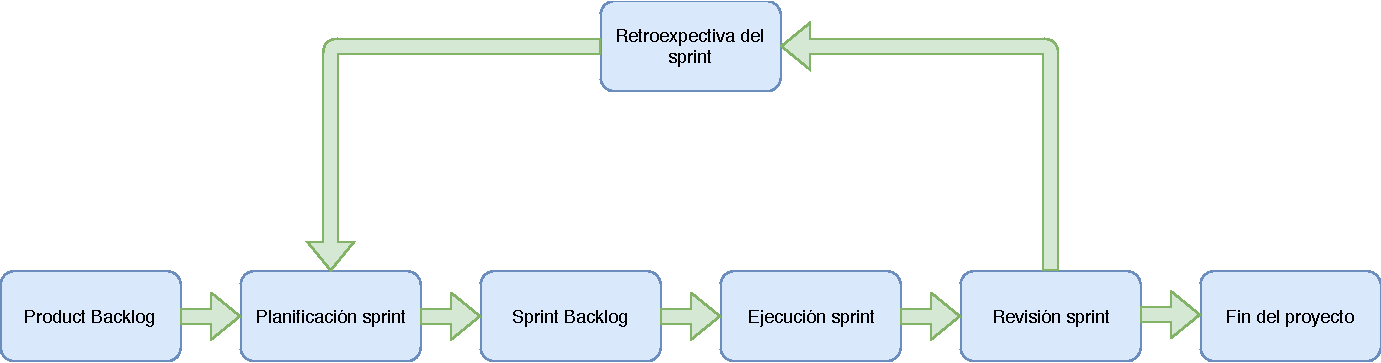
\includegraphics[width=0.4\linewidth]{Scrum}
  \caption[Desarrollo herramienta web]{Desarrollo herramienta web}
  \label{fig:Desarrollo herramienta web}
\end{figure}

Para este proyecto se han utilizado sprints de 30 días para asegurar el cumplimiento de estos.
 La distribución del tiempo fue de 75\% para realizar tareas del sprint en manera de cola de
 prioridad. Dentro de estas tareas se incluye el desarrollo de las pruebas necesarias y la
 comprobación de funcionalidades de las mismas. El resto 25\% se utilizó para el estudio del
 actual sprint para mejora de los siguientes, planificación y organización del siguiente sprint.
 En el capítulo de evaluación encontraremos la tabla con los sprints realizados y la funcionalidad
 desarrollada dentro de este.

\subsubsection{Definición de elementos}

Para la comprensión y buen desarrollo de esta metodología hace falta definir una serie
 de elementos los cuales son los siguientes:

\begin{itemize}
  \item \textbf{Product Backlog:} Será una lista de todos los requisitos del sistema, también
     conocido como historias de usuario. Estos requisitos estarán descritos en alto nivel
     de modo que cualquiera pueda entenderlo y estos estarán priorizados. Esta lista
     podrá verse modificada una vez iniciado el proyecto y en cualquier momento del ciclo de vida.
  \item \textbf{Sprint Backlog:} Esta será la lista de tareas a desarrollar durante el sprint
     para poder llegar al incremento planificado. Cada tarea deberá tener un tiempo estimado
     y los recursos que se necesitan para llevarlas a cabo. Cada tarea no deberá tener una
     estimación mayor de 24 horas puesto que esto indicaría que es demasiado larga y podría
     complicar el cumplimiento del resto de tareas para la fecha acordada. En caso de que
     alguna tarea supere dicho tiempo deberá ser dividida en subtareas.
  \item \textbf{Incremento:} Será el resultado esperado y obtenido al finalizar el sprint. Dicho
     resultado deberá ser terminado y poder ser utilizado.
\end{itemize}

En el caso de este proyecto, el producto backlog estará compuesto desde el principio de todas
 las funcionalidades que se desean implementar. Estas fueron obtenidas a raíz de la metodología
 de desarrollo. Para obtener mayor información sobre dichas funcionalidades deberemos consultar
 el siguiente capítulo en el cual se hablan de las mismas en profundidad.

Estas funcionalidades no serán las únicas en el product backlog puesto que durante el desarrollo
 e implementación del proyecto pueden surgir nuevas que no se hayan identificado en la etapa
 de captura de requisitios. Este caso ocurrio con el desarrollo del manual de usuario,
 informes para mostrar los resultados obtenidos y pequeñas mejoras identificadas al entregar
 el producto al final de cada sprint.

\subsubsection{Definición de roles}

 de personas tendrán los siguientes roles:
Dentro de un equipo que trabaje en esta metodología habrá dos grupos de personas. El primer grupo

\begin{itemize}
  \item \textbf{Product Owner:} Será el encargado de dar voz al cliente. En el caerá la
     responsabilidad de escribir las historias de usuario y ordenarlas en el product backlog.
   \item \textbf{Scrum Master:} Será el encargado de asegurarse que todo va bien en cuanto
      al proceso de desarrollo y este se cumple. Además intentará, en la medida de lo posible,
      evitar el mayor número de incidencias posibles.
   \item \textbf{Equipo:} Serán aquellos que se encarguen de realizar el desarrollo del producto.
\end{itemize}

En este proyecto el tutor del trabajo de fin de grado será quien adopte el rol de product owner
 y scrum master, mientras que el alumno ha sido formado por el autor del proyecto.

El otro grupo no entrará direcamente como parte del proceso, pero habrá que tenerlos en
 cuenta ya que serán ellos quienes nos den información al finalizar el sprint. De esta
 información podremos mejorar nuestro producto, aunque esto conllevará cambios en los
 siguientes sprints. Los usuarios que están dentro de este grupo serán aquellos que usen
 la herramienta, el usuario final. En nuestro caso serán los entrenadores y esgrimistas
 durante las competiciones o entrenamientos.

\subsubsection{Definición de reuniones}

Dentro de scrum existen diferentes tipos de reuniones. Estas reuniones son utilizadas para
 planificar las tareas del sprint, analizar las nuevas tareas que se han de incorporar en
 el product backlog, seguir el estado de salud del sprint y también comprobar cuales fueron
 los resultados de los sprints. Las diferentes reuniones que se llevan a cabo son las siguientes:

\begin{itemize}
  \item \textbf{Planificación del sprint:} En esta reunión se eligen las tareas del product
     backlog según estén ordenadas para mantener la prioridad de estas. Estas tareas deberán
     estar estimadas y hacerlo en caso de que no lo estén. En función del tiempo y recursos
     disponibles para el sprint se deberán escoger mas o menos tareas. Una vez seleccionadas
     tendremos el sprint backlog.
  \item \textbf{Seguimiento del sprint:} Esta será una reunión diaria de muy corta duración.
     El principal objetivo de esta reunión será conocer el estado de salud del sprint, de modo
     que se puedan tomar las medidas oportunas para que todo el trabajo salga adelante. Un
     claro ejemplo sería un bloqueo entre recursos que no se ha detectado previamente. Para
     ello cada miembro del equipo deberá comentar por encima cual fue su trabajo del día
     anterior junto con lo que tiene previsto para la jornada actual. No se deberán abordar
     problemas en esta reunión, sí se hará fuera de esta. Esta reunión es solo para estar al
     tanto de los posibles problemas.
  \item \textbf{Revisión del sprint:} En esta reunión se revisará el trabajo realizado y cuál
     faltó por completar. Además se presentará el incremento obtenido y se analizará el motivo
     de aquellas tareas que no se terminaron.
\end{itemize}


\subsection{Ciclo de vida SCRUM}

El ciclo de vida de SCRUM está formado por cinco fases, dichas fases son: concepto, especulación,
 exploración, revisión y cierre. A continuación se explican con mas detalle.

\begin{itemize}
  \item \textbf{Concepto:} Esta será la primera fase del ciclo de vida. Aquí será donde se sacará
     una primera idea sobre el producto realizada por el el cliente. También se definirá el alcance
     y el equipo de trabajo.
  \item \textbf{Especulación:} Una vez definido el alcance y con una visión del producto, se lanzarán
     hipotesis sobre lo que se desea obtener. Una vez lanzadas, se tendrá que hacer un contraste
     con la realidad. Esta fase se llevará a cabo en todas y cada una de las iteraciones del desarrollo.
  \item \textbf{Exploración:} Aquí será donde se lleven a cabo los incrementos del producto mediante
     el desarrollo de las funcionalidades definidas.
  \item \textbf{Revisión:} En esta fase se comprobará que se lleva a cabo la visión del producto, además
     de los objetivos que se han marcado para él.
  \item \textbf{Cierre:} Esta será la fase final del ciclo repetitivo, en la que se entregará
     el producto listo, funcional y revisado.
\end{itemize}

\textbf{Concepto}

Aquí definimos que producto queremos conseguir y como queremos conseguirlo. En este caso
 nuestro objetivo es elaborar una herramienta que permita apoyar a la decisión de una táctica
 en un asalto de esgrima. Para ello se optará por una aplicación web en la que puedas
 introducir los datos de los tiradores y que te aconseje sobre las acciones que debes o no
 hacer. Para ello deberá cumplir con tener una interfaz amigable, fácil y rápida de usar puesto
 que se usará en momentos de inquietud.

\textbf{Especulación}

En el caso de este proyecto las hipotesis lanzadas fueron transformadas a funcionalidades
 para una mayor visibilidad y comprensión de las mismas. Estas funcionalidades se han descrito
 mediante casos de uso. Dichos casos de uso se analizaron al comiendo del proyecto. Además, al
 finalizar cada sprint, después de un análisis, se incluyeron mejoras para el proyecto.

\textbf{Exploración}

Para la implementación de las funcionalidades deseadas se ha utilizado el paradigma de orientación a objetos
 usando un patrón de programación Modelo-Vista-Controlador. Esta es una de las
 razones por la que se eligió el lenguaje Ruby, ya que
 fue diseñado específicamente para ello. Además, es el más utilizado en dicho paradigma para el
 desarrollo de aplicaciiones web de desarrollo ágil. En concreto sacaremos especial partido
 a la parte de Vista-Controlador puesto que serán los controladores los que se encarguen de
 toda la lógica de la aplicación, entre ella estará el sistema experto y las decisiones que se toman.
 Las vistas serán las que se encarguen de recoger la información y enviarla a los controladores.
 Una vez que estos han procesado los datos y tienen un veredicto, de nuevo las vistas serán
 quienes tendrán la responsabilidad de mostrar los resultados de una manera entendible y
 de visionado rápido al usuario.

\textbf{Revisión}

En esta fase se fijarán las reuiones de fin de sprint, en las cuales se verificará que se
 han alcanzado todos los objetivos puestos para el sprint. También se comprobará que el producto
 se adecua a las funcionalidades que se planificaron.

\textbf{Cierre}

Esta será la fase en la que se hizo entrega del producto. Para ello tuvo que terminarse
 la implementación y aceptación de todas las funcionalidades que se describieron al inicio
 del proyecto, establecidas en el product backlog. Tener en cuenta que también han de cumplir
 lo anterior aquellas mejoras propuestas durante el desarrollo del proyecto.

La herramienta actualmente está en estado de mantenimiento, con lo cual se seguirá mejorando
 mediante nuevas funcionalidades propuestas por los usuarios de esta misma que pueden enviar
 en la propia herramienta.

\subsection{Validación}

Para la validación y adecuación de la herramienta desarrollada se han realizado una serie de
 tests unitarios los cuales comprobarán que el resultado de la funcionalidad es el esperado.
 Además se expondrá a diferentes usuarios los cuales nos darán su opinión y se analizará
 el uso que hacen sobre la herramienta para asegurar la facilidad de uso de la misma.

\subsection{Fases dentro del desarrollo}

Siguiendo SCRUM como metodología habrá unas series de fases que deberemos seguir para
 el obtener una mayor probabilidad de éxito dentro del desarrollo del proyecto. Como se
 mencionó anteriormente se definen unas series de tareas y se desarrollan según la prioridad
 que tengan estas. No todas las tareas que tengamos serán de desarrollar código, puesto
 que en algunas de ellas tendremos que hacer otros desempeños ya sean análisis de ciertas
 funcionalidades o investigación sobre algún tema para ver como se implementará cierta
 funcinoalidad. Las fases que han de seguirse son:

\begin{itemize}
  \item \textbf{Análisis:} Esta será la primera fase que tendremos que hacer ante cualquier tarea.
     Aquí será donde comprenderemos la índole de la tarea que tendremos que llevar a cabo. Para ello
     se investigará lo que sea necesario para comprender cual es el problema a resolver en la tarea
     y el motivo para resolverlo. En esta etapa será donde resolvamos la pregunta al QUE vamos
     a hacer. En este proyecto dichos análisis tendrán como resultado diagramas de casos de uso, los
     cuales serán representarán la manera en la que un usuario interactua con la aplicación. Además
     de lo mencionado anteriormente nos ayudará a visualizar la manera y orden en la que interactuan
     los elementos. Dentro de un diagrama de casos de uso podemos encontrar actores (usuarios en nuestro caso),
     casos de uso y relaciones entre los elementos. En la figura 3.3 se puede ver un caso
     de uso de ejemplo.

     \begin{figure}[htb]
       \centering
       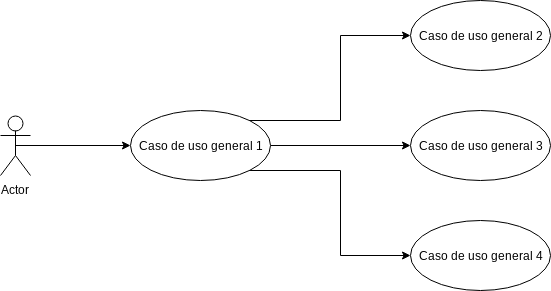
\includegraphics[width=0.4\linewidth]{diagramaCasoUsoGeneral}
       \caption[Ejemplo caso de uso general]{Ejemplo caso de uso general}
       \label{fig:blancoValido}
     \end{figure}

   \newpage

  \item \textbf{Diseño:} Cuando ya hemos conseguido saber con certeza que queremos hacer en la tarea
     pasaremos al COMO hacerlo. Para ello usaremos diagramas de secuencia. En dichos diagramas se podrán
     ver los pasos que se llevan a cabo para realizar una tarea, en nuestro caso será la implementación de un
     caso de uso. Dentro de un diagrama de secuencia podremos encontrar los elementos que componene el sistema
     e intervienen dentro de la funcionalidad a desarrolladas, los cuales estarán relacionados entre sí mediante
     líneas de secuencia. Con dichas líneas podremos obtener la información sobre el orden de los pasos que
     se llevan a cabo dentro de la funcionalidad. En la figura 3.4 se puede ver un diagrama de secuencia de
     ejemplo en el cual un actor es el que inicia una acción y esta conlleva que diferentes acciones se disparen.

     \begin{figure}[htb]
       \centering
       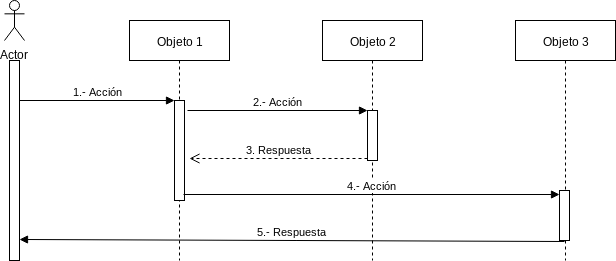
\includegraphics[width=0.4\linewidth]{diagramaSecuenciaGeneral}
       \caption[Ejemplo diagrama secuencia]{Ejemplo diagrama secuencia}
       \label{fig:blancoValido}
     \end{figure}

\end{itemize}
